\documentclass{beamer}
%
% Choose how your presentation looks.
%
% For more themes, color themes and font themes, see:
% http://deic.uab.es/~iblanes/beamer_gallery/index_by_theme.html
%
\mode<presentation>
{
  \usetheme{default}      % or try Darmstadt, Madrid, Warsaw, ...
  \usecolortheme{default} % or try albatross, beaver, crane, ...
  \usefonttheme{default}  % or try serif, structurebold, ...
  \setbeamertemplate{navigation symbols}{}
  \setbeamertemplate{caption}[numbered]
} 

\usepackage[english]{babel}
\usepackage[utf8]{inputenc}
\usepackage[T1]{fontenc}

\title[Paper and Issues]{Advances - Paper and Issues}
\author{Ricardo}
\institute{}
\date{\today}

\begin{document}

\begin{frame}
  \titlepage
\end{frame}

% Uncomment these lines for an automatically generated outline.
%\begin{frame}{Outline}
%  \tableofcontents
%\end{frame}


\begin{frame}{Problems}

\begin{itemize}
    \item Last paper rejected
    \pause 
    \item Some reasons: "Results not too high", "the work doesn't facilities a way to reproduce the results"
    
\end{itemize}
\onslide<2->{
\begin{block}{Taken Actions:}

\begin{itemize}
    \item Improve Nuclei Detection in high pleomorphism nuclei to improve our Characterization and knowledge
    
\end{itemize}

\end{block}}

\end{frame}


\begin{frame}{Improving Nuclei Detection in My Dataset}

\begin{itemize}

\item Using an Totally unsupervised method based on a Noiselet Characterization to enhance nuclei pleomorphism detection this was proved in some cases (a fast test)

\end{itemize}

\end{frame}


\begin{frame}{Pipeline}
\begin{columns}

\begin{column}{0.5\textwidth}
    
    \begin{itemize}
        \item<1-> \tiny Noiselet Extraction on tiles from the Hematoxylin image using patches of 2x2,4x4, 8x8 pixels (Scales)
        \item<2-> \tiny Using a K-means, 3 Clusters were computed over the features in each one of the different scales independly
        
        \item<3-> \tiny A image of Noise is obtained
        
        \item<4-> \tiny Determine the biggest area of noise in the binary image to be removed
        
        \item<5-> \tiny The image is intercepted with others computed equal but at different scales (\textbf{Final Noise Region})
        
        \item<6-> \tiny The Final Noise Region is removed from the H image and then is blurred 
         
        \item<8-> \tiny Nuclei detection with watershed
    \end{itemize}

\end{column}
    \begin{column}{0.5\textwidth}
    \only<1>{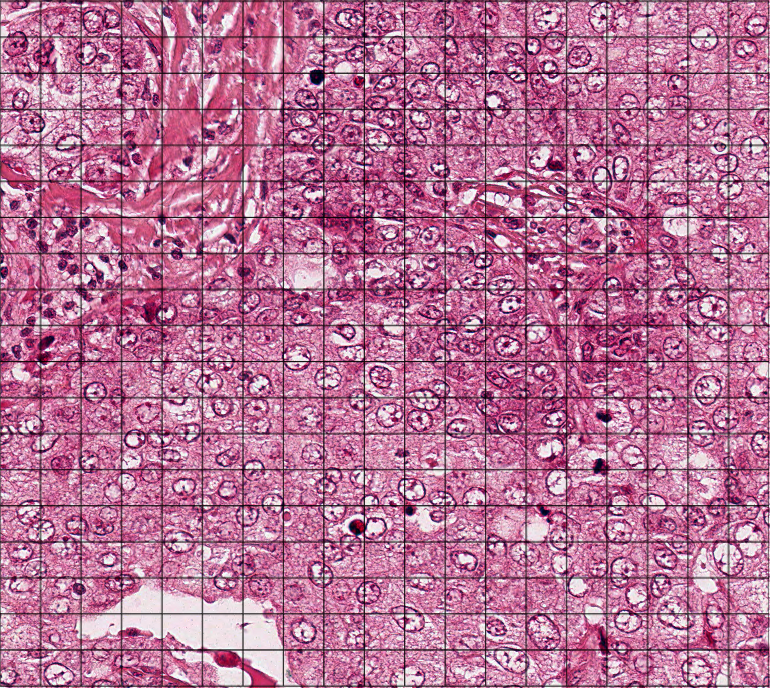
\includegraphics[width=\textwidth]{Process/grid.png}\\ 
    }
    \only<2>{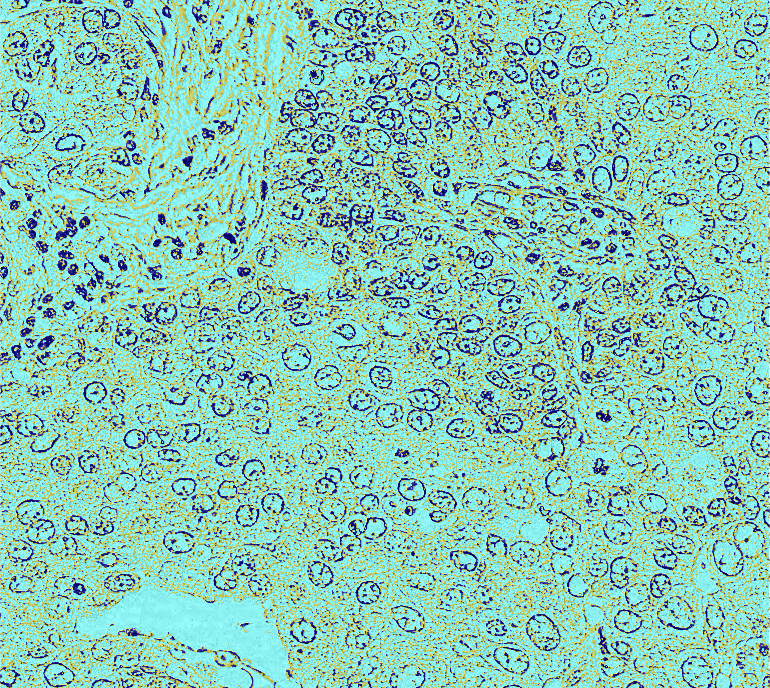
\includegraphics[width=\textwidth]{Process/Kmeans.png}
    }
\only<3>{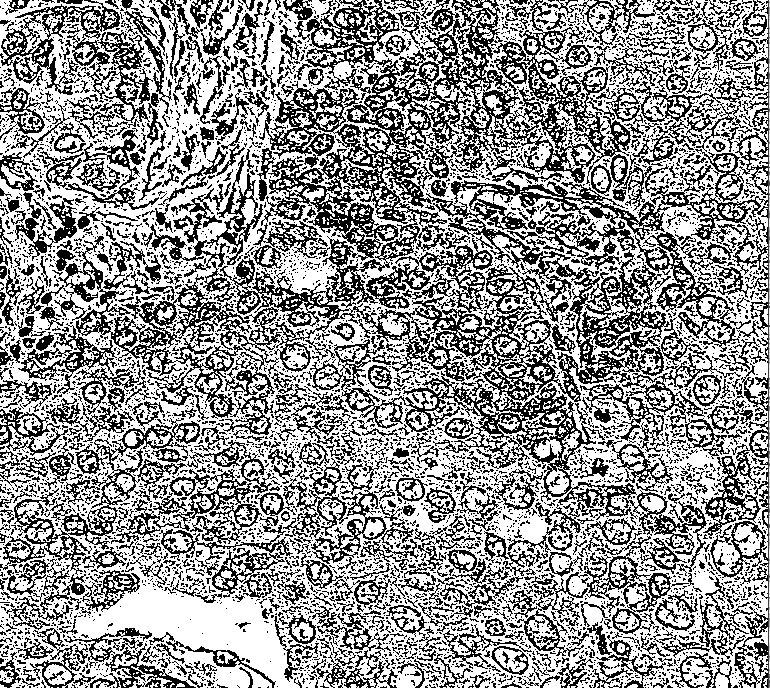
\includegraphics[width=\textwidth]{Process/AllNoise.png}
    }
    \only<4>{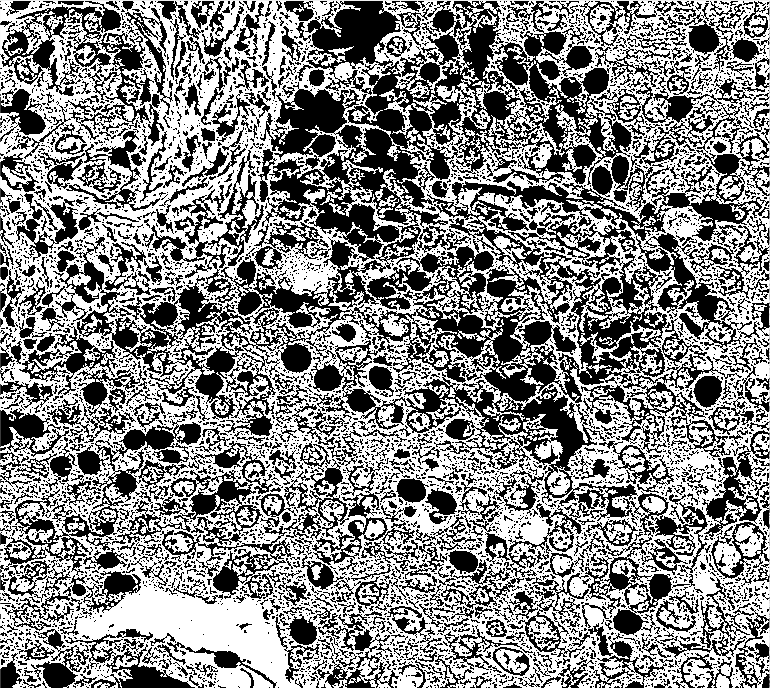
\includegraphics[width=\textwidth]{Process/BigNoise.png}
    }
            
    \only<5>{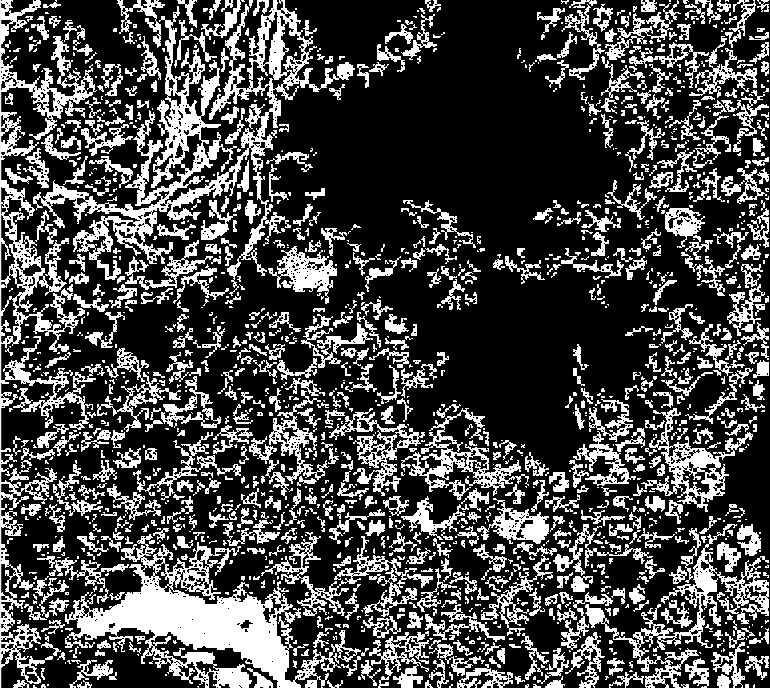
\includegraphics[width=\textwidth]{Process/ANDNoise.png}
    }
      
          \only<6>{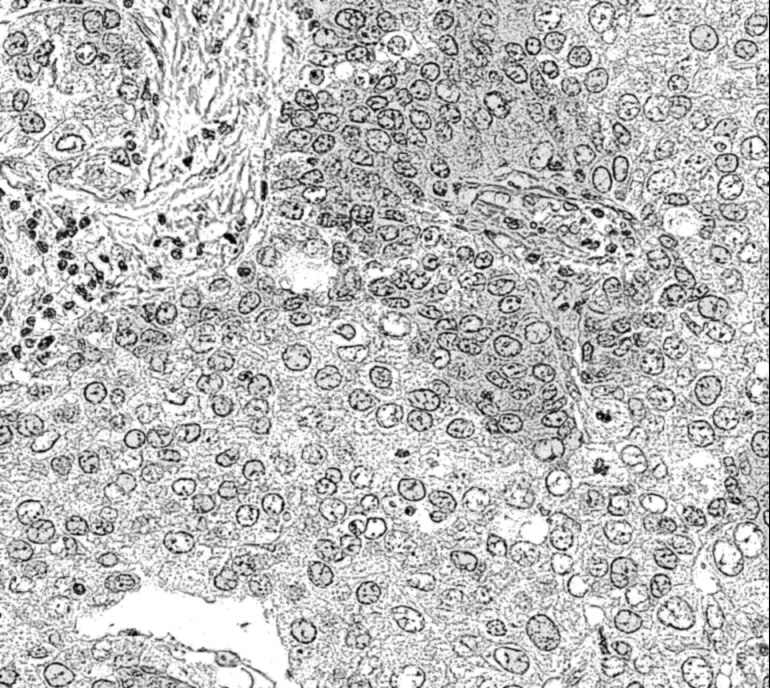
\includegraphics[width=\textwidth]{Process/FinalBlurred.png}\\ \centering Without Noise
    }
    \only<7>{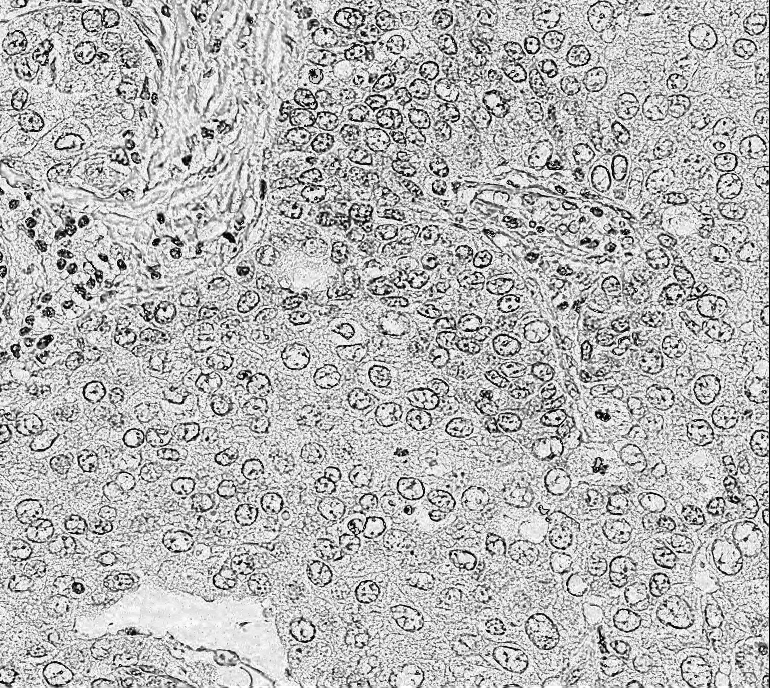
\includegraphics[width=\textwidth]{Process/OriginalH.png} \\ \centering With Noise
    }
                  

\end{column}
\end{columns}


\end{frame}


\begin{frame}{Visual Results }

\begin{columns}
    \begin{column}{0.5\textwidth}
    \centering Original Detection
    \only<1>{\includegraphics[width=\textwidth]{ResultsImgs/Exp1_original.png}
    False Nuclei
    }
    \only<2>{\includegraphics[width=\textwidth]{ResultsImgs/Exp2_original.png}
    Pleomorphic Nuclei Missing
    }
    \only<3>{\includegraphics[width=\textwidth]{ResultsImgs/Exp3_original.png}
    
    }
    
    \end{column}
    
    \begin{column}{0.5\textwidth}
    \centering After Method
        \only<1>{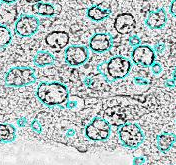
\includegraphics[width=\textwidth]{ResultsImgs/EXP1_Result.png}
        More True Nuclei Than False
    }
    \only<2>{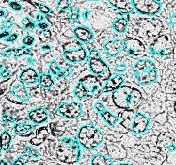
\includegraphics[width=\textwidth]{ResultsImgs/EXP2_Result.png}
    A better pleomorphism Capture
    }
    \only<3>{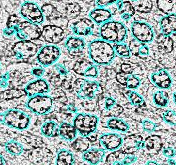
\includegraphics[width=\textwidth]{ResultsImgs/EXP3_Result.png}
    }
    
    \end{column}
\end{columns}
  \only<3>{\centering    Miss 6 Nuclei But 7 more were detected o improved}

    
\end{frame}


\begin{frame}{Discussion}
    \begin{itemize}
        \item The method can be much better
        \item Promising Results, needs to be writted
        \item For sure will increase the pleomorphism grading but maybe is not the time to include it
    \end{itemize}
\end{frame}


























\end{document}
